\chapter{Utvrđivanje autorstva}
U svijetu u kojem ne postoje unaprijed određena pravila pisanja programskog koda možemo pretpostaviti da svaki programer ostavlja svoj jedinstveni otisak dok programira. Cilj nam je kreirati klasifikator koji bi nam mogao odvojiti autore prema njihovom stilu programiranja. Ovakav klasifikator bi bilo moguće primjeniti na raznim open source projektima na kojima autori razvijaju kod anonimno te bi takav klasifikator mogao narušiti privatnost programera, ali ipak u ovom radu veći naglasak dan je na detekciju plagijata izvornih kodova te ovakav klasifikator koristimo za utvrđivanje autorstva na laboratorijskim vježbama ili na programerskim natjecanjima gdje su nam poznati neki identifikatori autora. \\

	Za rješavanje ovog problema korišteno je strojno učenje. Strojno učenje je grana umjetne inteligencije koja se bavi algoritmima koji mogu učiti na i raditi predviđanja nad skupovima podataka \cite{ml-def}. Postoje dvije vrste učenja, učenje pod nadzorom i učenje bez nadzora. Za učenje pod nadzorom potrebni su labelirani podaci te ih učimo kategorizirati, dok učenje bez nadzora pokušava uočiti uzorke iz podataka bez korištenja labela. Korišteno je nadzirano učenje gdje su podaci izvorni kodovi, a labele autori koji su ih napisali.  Konkretno, korišten je klasifikator slučajne šume. Konfiguracija i definicija klasifikatora je detaljnije opisana u \ref{sec:rf}. Klasifikacija je postupak u kojem određujemo kojoj kategoriji (od unaprijed određenih) novi podaci pripadaju. Algoritmi strojnog učenja ulazne podatke primaju u obliku brojeva pa je potrebno izvorni kod pretvoriti u vektor u kojem će svaki broj biti neka od značajki. Što bolje značajke odaberemo algoritam će bolje moći odvajati kategorije tj. autore. Skup odabranih značajki reflektira stil kojim programer piše kod te je nastao po uzoru na \cite{islam}. Skup značajki je podijeljen na leksičke, sintaksne i strukturalne.  Leksičke i strukturalne značajke dobijemo parsiranjem izvornog koda, a sintaksne iz apstraktnog sintaksnog stabla te je postupak izvlačenja detaljnije opisan \ref{sec:fe}. Na kraju poglavlja \ref{results} predstavljeni su i rezultati nad dva skupa izvornih kodova.

\section{Izvlačenje značajki} \label{sec:fe}
Kao što je već spomenuto, kako bi algoritmi strojnog učenja radili potrebni su im brojčani podaci kao ulazi. Izvorni kod se u brojčani vektor značajki pretvara koristeći ideju prvi put opisanu u radu \cite{islam}, a ideja je da se izvorni kod pretvori u vektor značajki sastavljen od tri dijela, leksičkog, sintaksnog i strukturnog. Leksičke i strukturalne značajke se dobiju izravno parsiranjem izvornog koda, dok nam je za sintaksne značajke potrebno apstraktno sintaksno stablo izvornog koda. Ovako definiran skup značajki je drugačiji za svaki pojedini programski jezik zbog različitosti među njima (npr. drugačije ključne riječi) te je potrebno napisati poseban parser za svaki od njih. U ovom radu naglasak je na programskom jeziku C++ te je izvlačenje značajki implementirano samo za njega. \\

	U nastavku su detaljno opisana i objašnjena sva tri tipa značajki. Većina tih značajki preuzeta je iz \cite{islam} dok su neke ideja samog autora. U većini značajki korištena je matematička operacija prirodnog logaritmiranja zbog svojstva da kako idemo prema većim vrijednostima ona sve manje i manje raste te dobro opisuje relativne razlike među značajkama. Neke od značajki su podijeljenje s duljinom izvornog koda kako bi bolje opisale frekvenciju pojavljivanja te značajke. 

\subsection{Leksičke značajke}
Leksičke značajke opisuju preferira li autor izvornog koda neke ključne riječi više od drugih(npr. for više od while), koristi li više funkcije ili piše monolitan kod, razne statistike(npr. prosječan broj parametara unutar funkcija), itd. Također izvorni kod se tokenizira te se računa frekvencija tako dobivenih tokena. \textit{Tablica} \ref{lexical} detaljno opisuje svaku od korištenih značajki. 

\subsection{Strukturne značajke}
Strukturne značajke opisuju kakvu strukturu autor koristi dok piše izvorni kod, npr. koristi li tabove ili razmake na početku linije, piše li novu liniju prije nego otvori kontrolni blok, itd. \textit{Tablica} \ref{layout} detaljno opisuje svaku od korištenih značajki.

\begin{table}[H]
\centering
\caption{Definicija leksičkih značajki}
\label{lexical}
\begin{adjustbox}{width=\textwidth, totalheight=\textheight,keepaspectratio}
\centering
\begin{tabular}{|l|l|l|l|}
\hline
\textbf{\textit{Ime značajke}}                 & \textbf{\textit{Definicija}}                                                                                                                              & \textbf{\textit{Izraz}}                       & \textbf{\textit{Veličina}}                                                                                             \\ \hline
Frekvencija unigrama           & \begin{tabular}[c]{@{}l@{}}Unigram definiramo kao jednu riječ\\  izvornog koda\end{tabular}                                             & UnigramFreq                 & \begin{tabular}[c]{@{}l@{}}dinamično, oko 20000 za 2160 \\ izvornih kodova (216 autora)\end{tabular} \\ \hline
Broj naredbi grananja i petlji & \begin{tabular}[c]{@{}l@{}}Zbroj svih pojavljivanja naredbi grananja\\ i petlji(for, while, do, if, else if, else, switch)\end{tabular} & ln(zbroj/duljina)           & 7                                                                                                    \\ \hline
Broj ključnih riječi           & \begin{tabular}[c]{@{}l@{}}Zbroj svih pojavljivanja ključnih riječi\\ programskog jezika, konkretno C++.\end{tabular}                   & ln(zbroj\_kljucne/duljina)  & 1                                                                                                    \\ \hline
Ternarni operatori             & Broj pojavljivanja ternarnog operatora                                                                                                  & ln(broj\_ternarnih/duljina) & 1                                                                                                    \\ \hline
Komentari                      & Broj pojavljivanja komentara                                                                                                            & ln(broj\_kom/duljina)       & 1                                                                                                    \\ \hline
Konstante                      & \begin{tabular}[c]{@{}l@{}}Broj pojavljivanja znakovnih i brojčanih \\ konstanti\end{tabular}                                           & ln(broj\_konst/duljina)     & 1                                                                                                    \\ \hline
Makro naredbe                  & Broj pojavljivanja makro naredbi                                                                                                        & ln(broj\_makro/duljina)     & 1                                                                                                    \\ \hline
Funkcije                       & Broj funkcija                                                                                                                           & ln(broj\_fun/duljina)       & 1                                                                                                    \\ \hline
Tokeni                         & \begin{tabular}[c]{@{}l@{}}Token je ekvivalentan unigramu, zbroj \\ svih tokena\end{tabular}                                            & ln(broj\_token/duljina)     & 1                                                                                                    \\ \hline
Mjere duljine linija           & \begin{tabular}[c]{@{}l@{}}Standardna devijacija i prosjek duljine \\ linija\end{tabular}                                               & stddev(linije), avg(linije) & 2                                                                                                    \\ \hline
Mjere parametara funkcija      & \begin{tabular}[c]{@{}l@{}}Standardna devijacija i prosjek broja \\ parametera funkcija\end{tabular}                                    & stddev(param), avg(param)   & 2                                                                                                    \\ \hline
Operatori                      & \begin{tabular}[c]{@{}l@{}}Zbroj pojavljivanja svih operatora \\ programskog jezika\end{tabular}                                        & ln(zbroj\_op/duljina)       & 1                                                                                                    \\ \hline
\end{tabular}
\end{adjustbox}
\end{table}


\begin{table}[H]
\centering
\caption{Definicija strukturnih značajki}
\label{layout}
\begin{adjustbox}{width=\textwidth, totalheight=\textheight,keepaspectratio}
\centering
\begin{tabular}{|l|l|l|l|}
\hline
\textbf{\textit{Ime značajke}}                 & \textbf{\textit{Definicija}}                                                                                                                              & \textbf{\textit{Izraz}}                       & \textbf{\textit{Veličina}}                                                                                             \\ \hline
Tabovi                                                                         & Broj svih tabova                                                                                  & ln(broj\_tabova/duljina)   & 1        \\ \hline
Razmaci                                                                        & Broj svih razmaka                                                                                 & ln(broj\_razmaka/duljina)  & 1        \\ \hline
Omjer razmaka                                                                  & \begin{tabular}[c]{@{}l@{}}Omjer razmaka(tabovi se broje) \\ i ostalih znakova\end{tabular}       & ln(zbroj\_kljucne/duljina) & 1        \\ \hline
\begin{tabular}[c]{@{}l@{}}Nova linija prije\\ vitičastih zagrada\end{tabular} & \begin{tabular}[c]{@{}l@{}}Koristi li autor novi red kada\\ otvara vitičastu zagradu\end{tabular} & boolean                    & 1        \\ \hline
\begin{tabular}[c]{@{}l@{}}Tabovi ili razmaci\\ na početku linije\end{tabular} & \begin{tabular}[c]{@{}l@{}}Koristi li autor tabove ili\\ razmake na početku linije\end{tabular}   & boolean                    & 1        \\ \hline
\end{tabular}
\end{adjustbox}
\end{table}


\subsection{Sintaksne značajke}
Sintaksne značajke se dobiju kako je već spomenuto iz apstraktnog sintaksnog stabla izvornog koda. One su što se vremena tiče najskuplje jer kreacija apstraktnih sintaksnih stabala nije brza, no trebale bi dati odlične značajke koje bi uvelike pomogle u deanonimizaciji. Apstraktna sintaksna stabla(ASS) su kreirana koristeći alat \textit{joern} \cite{joern}. Ovaj alat nudi posebnu skriptu \textit{joern-parse} koja parsira i vraća čvorove i bridove apstraktnog sintaksnog stabla. Postoji 58 različitih tipova čvorova(detalji u dodatku A) koje definira \textit{joern}.\textit{Tablica} \ref{syntax} detaljno opisuje svaku od korištenih značajki.

\begin{table}[H]
\centering
\caption{Definicija sintaksnih značajki}
\label{syntax}
\begin{adjustbox}{width=\textwidth, totalheight=\textheight,keepaspectratio}
\centering
\begin{tabular}{|l|l|l|l|}
\hline
\textit{\textbf{Ime značajke}}                                    & \textit{\textbf{Definicija}}                                                                     & \textit{\textbf{Izraz}} & \textit{\textbf{Veličina}}                                                                \\ \hline
Bigrami  čvorova                                                  & \begin{tabular}[c]{@{}l@{}}Bigrami čvorova su dva čvora \\ koja su povezana u ASS-u\end{tabular} & bigrami\_čvorovaTF      & \begin{tabular}[c]{@{}l@{}}dinamičko, oko 150000 za 2160 \\ izvornih kodova\end{tabular}  \\ \hline
Tip čvora ASS-a                                                   & \begin{tabular}[c]{@{}l@{}}Frekvencija pojavljivanja tipa\\ čvora ASS-a\end{tabular}             & tip\_čvoraTF            & 58                                                                                        \\ \hline
\begin{tabular}[c]{@{}l@{}}Vrijednost lista \\ ASS-a\end{tabular} & \begin{tabular}[c]{@{}l@{}}Frekvencija vrijednosti listova\\ ASS-a\end{tabular}                  & list\_vTF               & \begin{tabular}[c]{@{}l@{}}dinamičko, oko 10000 za 2160\\ izvornih kodova\end{tabular} \\ \hline

\end{tabular}
\end{adjustbox}
\end{table}


\section{Selekcija značajki}
Ovako kreirane značajke rezultiraju u ogromnim, rijetkim (eng.~ \textit{sparse}) vektorima, čija veličina nekada doseže i stotine tisuća brojeva. Razlog tomu leži u definiciji značajki poput frekvencije tokena, frekvencije bigrama, itd. Rijetkost očitujemo u velikom broju nula unutar vektora. Rijetkost, također, može uzrokovati loš izabir idućeg čvora u klasifikatoru slučajne šume te s time i lošije rezultate. S velikim vektorima također dolazi i do puno sporijeg učenja klasifikatora jer će sva stabla odluka unutar slučajne šume imati više čvorova. Zbog svih navedenih razloga prije samog učenja klasifikatora napravljena je selekcija značajki koja odabire manji broj značajki koje sadrže dovoljno informacija da bi se klasifikator bolje i brže naučio. Tehnika selekcije značajki je mnogo pa se detaljnije ulazi samo u one koje su korištene u ovom radu, a to su selekcija značajki po sadržaju informacije te selekcija značajki po iznosu varijance. Više o rezultatima sa i bez selekcije značajki u poglavlju \ref{results}.

\subsection{Selekcija značajki po sadržaju informacije}

Svaka pojedinačna značajka vektora značajki nosi sa sobom neku količinu ili sadržaj informacije(eng. \textit{information gain}), te nam ona govori koliko je ta značajka bitna za klasifikaciju. Selektiramo samo one značajke koje sa sobom nose najveći sadržaj informacije. Definicija sadržaja informacije je detaljnije opisana u \ref{entropy}.

\subsection{Selekcija značajki po iznosu varijance}

Značajke su brojevi pa nad njima možemo računati razne statistike pa tako i varijancu. Ova selekcija značajki odbacuje sve značajke koje ne pređu unaprijed određenu granicu(eng. \textit{threshold}) iznosa varijance.

\section{Slučajna šuma} \label{sec:rf}

Slučajna šuma \cite{breiman} je klasifikator koji se sastoji od kolekcije nezavisnih stabala odlučivanja. Svako od stabala predstavlja jedan glas u većinskom donošenju odluke. Odluka se donosi zbrajanjem glasova te se odabire odluka s najvećim brojem glasova \cite{rfdef}. Ovo detaljnije možemo vidjeti na slici \ref{fig:rf}. Slučajna šuma jer je u svojoj osnovi samo skup stabala vrlo dobro podnosi veliku dimenzionalnost podataka (što za ovaj problem očekujemo) i ne očekuje linearnu odvojivost vektora značajki te je iz tih razloga odabrana kao korišteni algoritam.  \\

\begin{figure}[H]
	\centering
	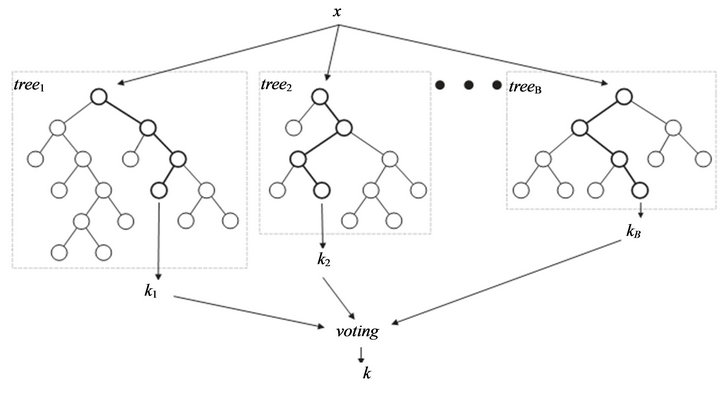
\includegraphics[width=0.8\textwidth]{fig/random-forest-overview.jpg}
	\caption{Arhitektura slučajne šume \cite{fig-rf}}
	\label{fig:rf}
\end{figure}

	
	Svako od N stabala odluke je izgrađeno nasumičnim uzorkovanjem s ponavljanjima skupa za treniranje tako da se uzorkuje podskup duljine \textit{N}. Stabla se grade do maksimalne moguće dubine iako postoje instance algoritma u kojem se stabla podrezuju. U izgradnji stabla ponovno se slučajno odabire podskup značajki kojih ima \textit{M}. Veličina tog podskupa je hiperparametar algoritma, u literaturi \cite{statisticallearning} se za klasifikacijski problem preporuča veličina od $\sqrt{M}$. Od tog podskupa treba odabrati najbolju značajku koja će biti iskorištena za idući čvor stabla. Odabir najbolje značajke uobičajeno se radi metodama Gini nečistoće ili uzajamnog sadržaja informacije.
	
\subsection{Gini nečistoća}

Gini nečistoća je mjera koliko često bi nasumično odabrana značajka iz nekog skupa bila krivo klasificirana ako bi ju se nasumično klasificiralo s obzirom na to kakva je razdioba značajki po razredima u podskupu svih značajki. Drugim riječima gini nečistoća je kriterij koji teži minimizaciji vjerojatnosti krive klasifikacije \cite{cse}. Računamo ju na sljedeći način \cite{gidef}:
\begin{equation}
	I_g(t) = 1 -  \sum_{i=1}^{c} p(i | t)^{2}
\end{equation}
gdje je $p(i | t)$ broj značajki koje pripadaju klasi \textit{i} za čvor \textit{t}. 

\subsection{Uzajamni sadržaj informacije} \label{entropy}

Uzajamni sadržaj informacije je koncept baziran na entropiji. Entropija je definirana kao količina informacije koju nosi neka poruka te ju računamo:
\begin{equation}
		H(t) = - \sum_{i} p(x_{i}) * log_2 p(x_{i})
\end{equation}
gdje su $p(x_{i})$ vjerojatnosti svake od klasa. \newline
Uzajamni sadržaj informacije definiran je kao:
\begin{equation}
		I(X;Y_{i}) = H(X) - H(X | Y_{i})
\end{equation}
gdje je \textit{X} klasa(autor), a $Y_{i}$ i-ta značajka iz skupa. Intuitivno ga možemo zamisliti kao količinu informacije koju daje značajka $i$ za klasu kojoj pripada.

\section{Prikupljanje podataka}
Izvorni kodovi korišteni u eksperimentima djelo su učenika srednjih i osnovih škola koji su se natjecali na HONI-u\footnote{http://www.hsin.hr/honi/} u godini 2016-2017. Skupljena su dva skupa podataka, jedan od 216 autora gdje svaki od njih ima 10 izvornih kodova i drugi od 29 autora s također 10 izvornih kodova. Razlika je u tome što su u većem skupu izvorni kodovi birani nasumično iz skupa svih rješenja autora, dok su u manjem skupu oni odabrani kao rješenja istih 10 zadataka. Cilj ovakvog odabira  je dobiti što objektivniju točnost naučenog klasifikatora. Oba skupa su dostupna na poveznici\footnote{https://dropbox.com} s dna stranice. HONI je odabran jer se činilo zanimljivo isprobati algoritam na domaćem natjecanju iako bi rezultati bilo vjerojatno bolji da se koristilo natjecanje poput Google Code Jam-a\footnote{\url{https://code.google.com/codejam/}} koje je znatno veće i nudi više mogućnosti. 

\section{Rezultati i rasprava} \label{results}

Napravljeno je nekoliko različitih eksperimenata s različitim hiperparametrima i selekcijom značajki kako bi dobili što bolju sliku kako algoritam radi. Svaki od eksperimenata je odrađen k-preklop među validacijom(eng. \textit{k-fold cross validation}), gdje je k u našem slučaju 10 jer imamo po 10 rješenja za svakog autora, kako bi dobili što objektivnije i točnije rezultate. U svakoj iteraciji 9 izvornih kodova autora birano je u skup za treniranje, a preostali izvorni kod u skup za testiranje. Svako od stabala unutar slučajne šume građeno je do samog kraja te je za odabir novog čvora korišteno $\sqrt{N}$ značajki kako je to preporučeno u \cite{statisticallearning}. Ovi hiperparametri su se pokazali daleko najboljima te ih nije bilo potrebe mijenjati te je jedini varijabilni hiperparametar bio broj drveća unutar slučajne šume. Također su prikazane po dvije slike za svaki eksperiment, jedna sa skupom od leksičkih i strukturnih značajki te jedna sa skupom leksičkih, strukturnih i sintaksnih značajki. To je napravljeno kako bi što bolje shvatili koliko su koje značajke bitne za prepoznavanje autora.

\subsection{Rezultati bez selekcije značajki}

U ovom poglavlju prikazani su  rezultati bez selekcije značajki. Krenulo se s pretpostavkom da će nam sintaksne značajke donijeti veliko poboljšanje klasifikatora što spominju i \cite{islam}, no kao što možemo vidjeti na slikama \ref{sve_znacajke} i \ref{leks_znacajke} sintaksne značajke nisu donijele veliko poboljšanje klasifikatora na manjem skupu autora, dok su na većem skupu autora ukupnu točnost čak dosta i smanjili. 

\begin{figure}[H]
  \centering
  \begin{minipage}[b]{0.49\textwidth}
    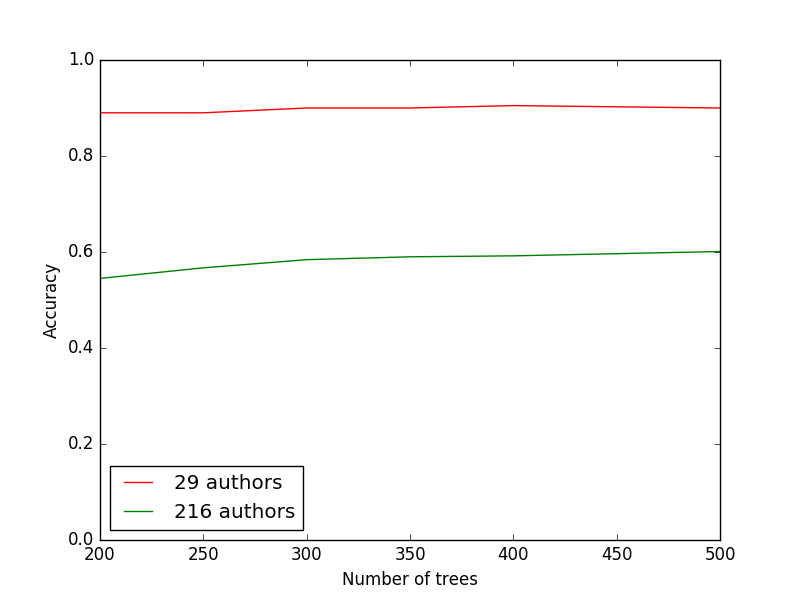
\includegraphics[width=\textwidth]{fig/sve_znacajke_bez_fs.png}
    \caption{Točnost klasifikatora uz leksičke, strukturne i sintaksne značajke}
    \label{sve_znacajke}
  \end{minipage}
  \hfill
  \begin{minipage}[b]{0.49\textwidth} 
    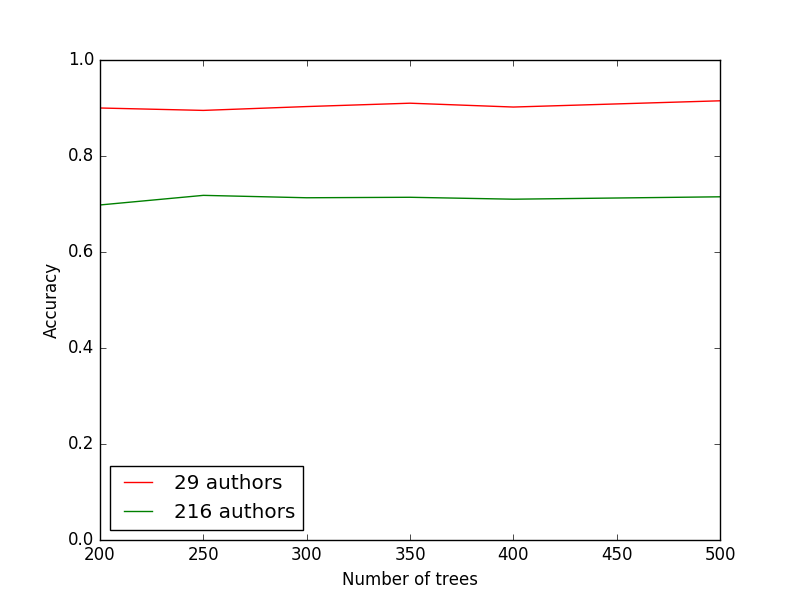
\includegraphics[width=\textwidth]{fig/leksicke_bez_fs.png}
    \caption{Točnost klasifikatora uz leksičke i strukturne značajke}
    \label{leks_znacajke}
  \end{minipage}
\end{figure}

\subsection{Rezultati uz selekciju značajki sadržajem informacije}

U ovom poglavlju predstavljam rezultate kada je korištena selekcija značajki uzajamni sadržajem informacije koja bi zbog prirode značajki koje su dosta rijetke trebala povećati točnost klasifikatora s obzirom na slučaj bez selekcije značajki što se doista i pokazalo istinito te to možemo vidjeti na slikama \ref{sve_znacajke_ig} i \ref{leksicke_ig}. Primjećujemo da su nam sintaksne značajke i u ovom slučaju donijele pogoršanje točnosti. \\
	Također pošto selekcija značajki smanjuje dimenzionalost vektora značajki sa stotina tisuća na desetke tisuća donosi nam veliko ubrzanje učenja klasifikatora.

\begin{figure}[H]
  \centering
  \begin{minipage}[b]{0.49\textwidth}
    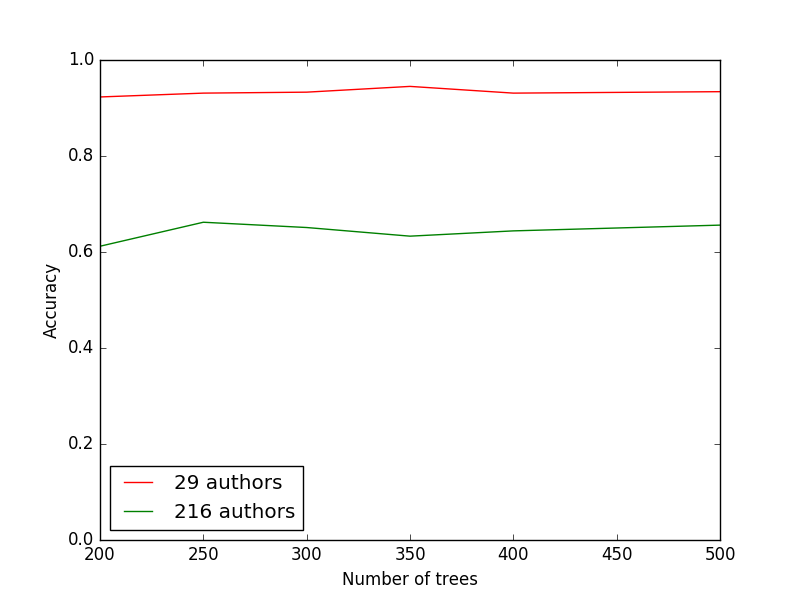
\includegraphics[width=\textwidth]{fig/ig_sve_znacajke.png}
    \caption{Točnost klasifikatora uz leksičke, strukturne i sintaksne značajke}
    \label{sve_znacajke_ig}
  \end{minipage}
  \hfill
  \begin{minipage}[b]{0.49\textwidth}
    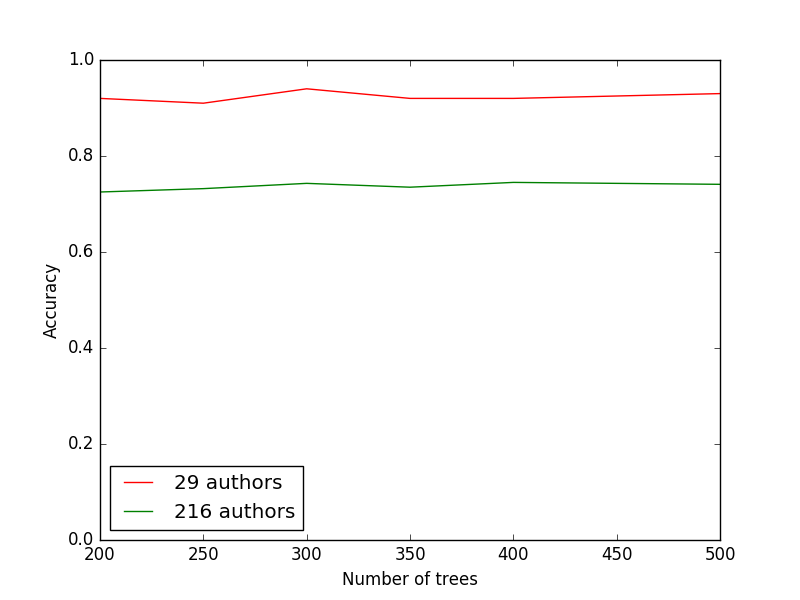
\includegraphics[width=\textwidth]{fig/leksicke_fs.png}
    \caption{Točnost klasifikatora uz leksičke i strukturne značajke}
    \label{leksicke_ig}
  \end{minipage}
\end{figure}

\subsection{Rezultati uz selekciju značajki varijancom}

U ovom poglavlju predstavljam rezultate korištenjem selekcije značajki varijancom, u eksperimentu je korištena granica varijance od $0.03$ jer je pokazala najbolje rezultate. Možemo primjetiti da su rezultati bolji nego kada smo koristili sve značajke, no lošiji su nego sa selekcijom uzajamnim sadržajem informacije što vidimo na slikama \ref{vt_sve} i \ref{vt_leksicke}.

\begin{figure}[H]
  \centering
  \begin{minipage}[b]{0.49\textwidth}
    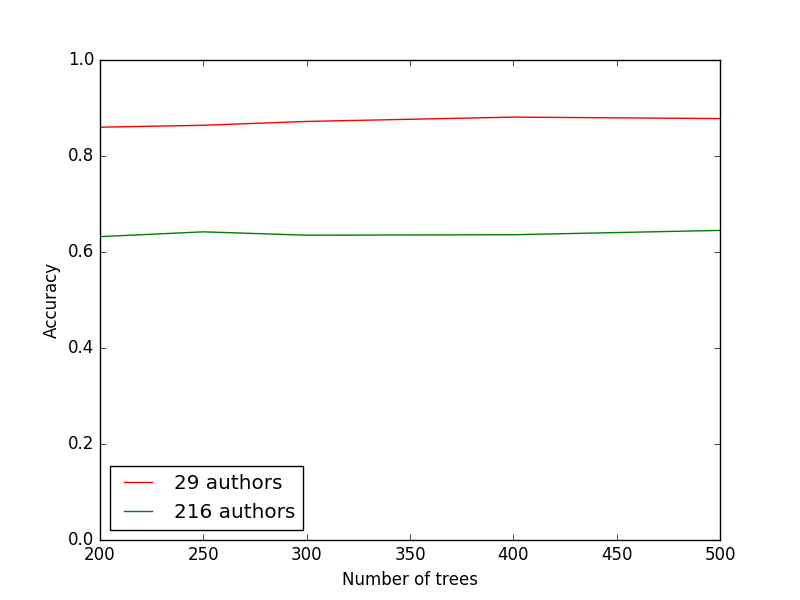
\includegraphics[width=\textwidth]{fig/vt_sve.png}
    \caption{Točnost klasifikatora uz leksičke, strukturne i sintaksne značajke}
    \label{vt_sve}
  \end{minipage}
  \hfill
  \begin{minipage}[b]{0.49\textwidth}
    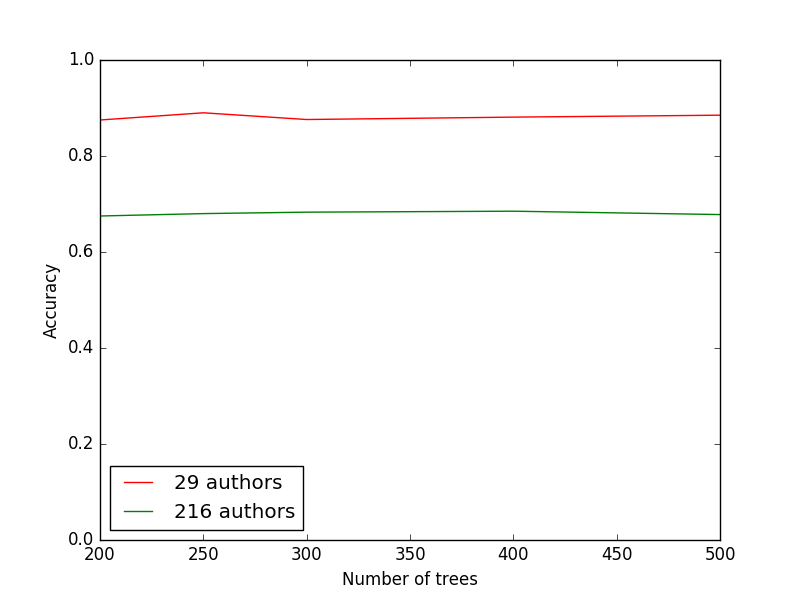
\includegraphics[width=\textwidth]{fig/leksicke_vt.png}
    \caption{Točnost klasifikatora uz leksičke i strukturne značajke}
    \label{vt_leksicke}
  \end{minipage}
\end{figure}

\subsection{Rasprava}

Prva stvar koju možemo primjetiti da što manji broj autora predamo klasifikatoru na treniranje to su nam rezultati bolji, što ima i smisla jer mora odlučiti na manjem broju kategorija, a ima jednako izvornih kodova za svakog autora kao u slučaju s velikim brojem autora. Sintaksne značajke nam uglavnom donose lošije rezultate nego što smo pretpostavljali te vidjeli u \cite{islam}. Dodatno one donose stotine tisuća značajki i znatno usporavaju treniranje te su iz tih razloga izbačene za potrebe web aplikacije $Turtle$. Kao zaključak naveo bih da su rezultati dovoljno dobri za potrebe detekcije plagijata, ali ipak nisu ni blizu rezultatima iz \cite{islam}. Može se primjetiti da se ovako definiran skup značajki izvornog koda može primjeniti na skoro svaki poznatiji programski jezik te bi to bilo zanimljivo isprobati u budućem radu.